% !TEX root = ../../../main.tex
% 所属：第一部分：单变量分析学 / 第2章：一元实函数与基本初等函数——你所应当知晓的
% 节：2.2 基本初等函数
% 正文按原文件顺序保存；由 ../chapter2.tex 调用。
\section{基本初等函数}
这一节介绍基本初等函数的一些常用的公式，它们可能是大学老师说的高中老师会讲，但高中老师说大学老师会讲的内容
\subsection*{代数恒等式}
\begin{proposition}[二项式定理]
	对任意 $n \in \N$，
	\[
	(x+y)^n = \sum_{k=0}^{n} \binom{n}{k} x^{n-k} y^k,
	\]
	其中 $\displaystyle\binom{n}{k} = \frac{n!}{k!(n-k)!}$ 为二项式系数。
\end{proposition}

\begin{proof}
	对 $n$ 用数学归纳法。$n=0$ 时 $(x+y)^0 = 1 = \binom{0}{0}x^0y^0$，成立。
	
	假设 $n$ 时成立，则
	\[
	\begin{aligned}
	(x+y)^{n+1} &= (x+y)(x+y)^n = (x+y)\sum_{k=0}^{n}\binom{n}{k}x^{n-k}y^k \\
	&= \sum_{k=0}^{n}\binom{n}{k}x^{n+1-k}y^k + \sum_{k=0}^{n}\binom{n}{k}x^{n-k}y^{k+1} \\
	&= x^{n+1} + \sum_{k=1}^{n}\left[\binom{n}{k}+\binom{n}{k-1}\right]x^{n+1-k}y^k + y^{n+1}.
	\end{aligned}
	\]
	由 Pascal 恒等式 $\binom{n}{k} + \binom{n}{k-1} = \binom{n+1}{k}$，即得 $n+1$ 时成立。
\end{proof}

\begin{proposition}[多项式定理]
	对任意 $n \in \N$，
	\[
	\left(\sum_{i=1}^{p} x_i\right)^n = \sum_{\substack{n_1+\cdots+n_p = n \\ n_1,\dots,n_p \in \N}} \binom{n}{n_1,\dots,n_p} \prod_{i=1}^{p} x_i^{n_i},
	\]
	其中 $\displaystyle\binom{n}{n_1,\dots,n_p} = \frac{n!}{n_1!\, n_2! \,\cdots\, n_p!}$ 为多项式系数。
\end{proposition}

\begin{proof}
	二项式定理的直接推广。展开乘积时，每一项对应从 $n$ 个因子中各选一个 $x_i$，$n_i$ 记录选取 $x_i$ 的次数。系数的组合意义即 $n$ 个元素中有 $n_i$ 个不可区分的第 $i$ 类元素时的排列数，由归纳法可严格证明。
\end{proof}

\begin{proposition}[平方差与 $n$ 次方差公式]
	对任意 $n \in \N$，$n \geqslant 1$，
	\[
	x^n - y^n = (x-y)(x^{n-1} + x^{n-2}y + \cdots + xy^{n-2} + y^{n-1}).
	\]
	当 $n$ 为奇数时，
	\[
	x^n + y^n = (x+y)(x^{n-1} - x^{n-2}y + \cdots - xy^{n-2} + y^{n-1}).
	\]
\end{proposition}

\begin{proof}
	对 $x^n - y^n$，将 $(x-y)$ 乘以右侧的几何级数和：
	\[
	\begin{aligned}
	(x-y)\sum_{k=0}^{n-1} x^{n-1-k}y^k &= \sum_{k=0}^{n-1} x^{n-k}y^k - \sum_{k=0}^{n-1} x^{n-1-k}y^{k+1} \\
	&= x^n + \sum_{k=1}^{n-1} x^{n-k}y^k - \sum_{k=0}^{n-2} x^{n-1-k}y^{k+1} - y^n = x^n - y^n.
	\end{aligned}
	\]
	当 $n$ 为奇数时，用 $-y$ 代入上式即得 $x^n + y^n = x^n - (-y)^n = (x+y)(\cdots)$。
\end{proof}

\begin{proposition}[前 $n$ 个正整数的方幂和]
	\[
	\sum_{k=1}^{n} k = \frac{n(n+1)}{2}, \qquad
	\sum_{k=1}^{n} k^2 = \frac{n(n+1)(2n+1)}{6}, \qquad
	\sum_{k=1}^{n} k^3 = \left[\frac{n(n+1)}{2}\right]^2.
	\]
\end{proposition}

\begin{proof}
	第一个公式：将 $S = 1+2+\cdots+n$ 倒序写为 $S = n+(n-1)+\cdots+1$，相加得 $2S = n(n+1)$。
	
	第二个公式：利用恒等式 $(k+1)^3 - k^3 = 3k^2 + 3k + 1$，对 $k=1$ 到 $n$ 求和：
	\[
	(n+1)^3 - 1 = 3\sum_{k=1}^{n} k^2 + 3\cdot\frac{n(n+1)}{2} + n,
	\]
	解得 $\sum k^2 = \dfrac{n(n+1)(2n+1)}{6}$。
	
	第三个公式：利用 $(k+1)^4 - k^4 = 4k^3 + 6k^2 + 4k + 1$ 求和，或注意到 $\sum k^3 = (\sum k)^2$，可由归纳法验证。
\end{proof}

\begin{proposition}[一元二次方程求根公式]
	方程 $ax^2 + bx + c = 0$（$a \neq 0$）的根为
	\[
	x_{1,2} = \frac{-b \pm \sqrt{b^2 - 4ac}}{2a}.
	\]
\end{proposition}

\begin{proof}
	配方：$a(x^2 + \frac{b}{a}x) + c = 0$，即 $a\left[(x+\frac{b}{2a})^2 - \frac{b^2}{4a^2}\right] + c = 0$，整理得 $(x+\frac{b}{2a})^2 = \frac{b^2-4ac}{4a^2}$，开方即得。
\end{proof}

\begin{proposition}[一元三次方程求根公式——Cardano 公式]
	考虑缺项三次方程
	\[
	t^3 + pt + q = 0,
	\]
	其中 $p, q \in \R$。令判别式 $\Delta = \left(\dfrac{q}{2}\right)^2 + \left(\dfrac{p}{3}\right)^3$。
	\begin{enumerate}
		\item 若 $\Delta > 0$，方程有一个实根和两个共轭复根：
		\[
		t_1 = u + v, \quad t_{2,3} = -\frac{u+v}{2} \pm i\frac{\sqrt{3}}{2}(u-v),
		\]
		其中 $u = \sqrt[3]{-\dfrac{q}{2} + \sqrt{\Delta}}$，$v = \sqrt[3]{-\dfrac{q}{2} - \sqrt{\Delta}}$。
		\item 若 $\Delta = 0$，三个实根（有重根）：
		\[
		t_1 = 2\sqrt[3]{-\frac{q}{2}}, \quad t_2 = t_3 = -\sqrt[3]{-\frac{q}{2}}.
		\]
		\item 若 $\Delta < 0$，三个互异实根（不可约情形），用三角形式表示：
		\[
		t_k = 2\sqrt{-\frac{p}{3}} \cos\left(\frac{1}{3}\arccos\left(\frac{-q/2}{\sqrt{-(p/3)^3}}\right) + \frac{2k\pi}{3}\right), \quad k = 0,1,2.
		\]
	\end{enumerate}
\end{proposition}

\begin{proof}
	设 $t = u + v$，则
	\[
	t^3 = (u+v)^3 = u^3 + v^3 + 3uv(u+v) = u^3 + v^3 + 3uv \cdot t.
	\]
	因此 $t^3 - 3uv \cdot t - (u^3+v^3) = 0$。与原方程 $t^3 + pt + q = 0$ 比较系数：
	\[
	uv = -\frac{p}{3}, \qquad u^3 + v^3 = -q.
	\]
	于是 $u^3$ 和 $v^3$ 是二次方程 $z^2 + qz - \left(\dfrac{p}{3}\right)^3 = 0$ 的两根，解得
	\[
	u^3, v^3 = -\frac{q}{2} \pm \sqrt{\left(\frac{q}{2}\right)^2 + \left(\frac{p}{3}\right)^3}.
	\]
	取 $u, v$ 满足 $uv = -p/3$（即 $uv$ 为实数），就得到 Cardano 公式。
	
	$\Delta < 0$ 时 $u, v$ 为共轭复数，用极坐标 $u = r e^{i\theta}$，$v = r e^{-i\theta}$，则 $t = u+v = 2r\cos\theta$，经计算得三角形式。
\end{proof}


	对一般三次方程 $ax^3 + bx^2 + cx + d = 0$（$a \neq 0$），先除以 $a$ 化为 $x^3 + Bx^2 + Cx + D = 0$，其中 $B = b/a$，$C = c/a$，$D = d/a$。作变量替换 $x = t - B/3$ 消去二次项，得
	\[
	t^3 + pt + q = 0, \qquad p = C - \frac{B^2}{3}, \quad q = \frac{2B^3}{27} - \frac{BC}{3} + D.
	\]
	求出 $t$ 后回代 $x = t - B/3$ 即得原方程的三根。



\subsection*{三角函数的基本公式}

我们假设读者已熟悉任意角弧度制下 $\sin x, \cos x, \tan x$ 等的几何定义以及诱导公式。以下 $x, y \in \R$，$n \in \N$。

\begin{proposition}[同角基本关系]
	\[
	\sin^2 x + \cos^2 x = 1, \quad
	1 + \tan^2 x = \sec^2 x, \quad
	1 + \cot^2 x = \csc^2 x.
	\]
	\[
	\tan x = \frac{\sin x}{\cos x}, \quad
	\cot x = \frac{\cos x}{\sin x}, \quad
	\sec x = \frac{1}{\cos x}, \quad
	\csc x = \frac{1}{\sin x}.
	\]
\end{proposition}

\begin{proof}
	在单位圆 $x^2+y^2=1$ 上，取角 $x$ 对应点 $(\cos x, \sin x)$，由定义直接得 $\sin^2 x + \cos^2 x = 1$。其余关系由定义出发，两边同除 $\cos^2 x$ 或 $\sin^2 x$ 即得。
\end{proof}

\begin{proposition}
	\[\begin{aligned}
		\sin(x \pm y) &= \sin x \cos y \pm \cos x \sin y, \\
		\cos(x \pm y) &= \cos x \cos y \mp \sin x \sin y, \\
		\tan(x \pm y) &= \frac{\tan x \pm \tan y}{1 \mp \tan x \tan y}.
	\end{aligned}\]
\end{proposition}
\begin{proof}
	用向量或几何方法证明余弦差公式。在单位圆上取点 $A(\cos x, \sin x)$，$B(\cos y, \sin y)$，如图所示：
	\begin{center}
	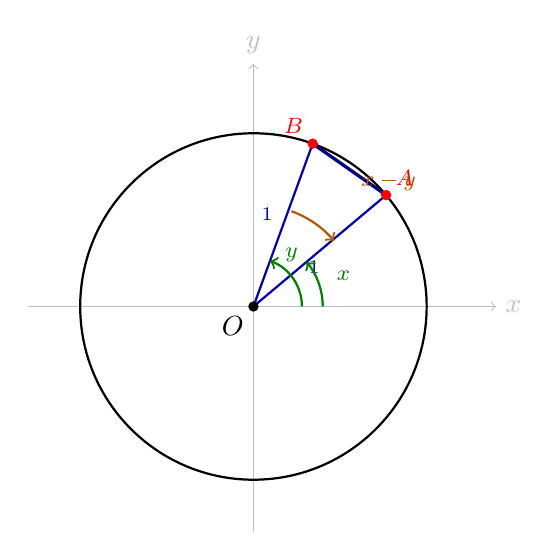
\begin{tikzpicture}[scale=2.2]
		% 坐标轴
		\draw[->, gray!50] (-1.3,0) -- (1.4,0) node[right] {$x$};
		\draw[->, gray!50] (0,-1.3) -- (0,1.4) node[above] {$y$};
		% 单位圆
		\draw[thick] (0,0) circle (1);
		% 点 A (角 x ~40°), B (角 y ~70°)
		\coordinate (A) at (0.766, 0.643);
		\coordinate (B) at (0.342, 0.940);
		% 半径 OA, OB
		\draw[thick, blue!70!black] (0,0) -- (A) node[midway, below, xshift=-2pt] {\scriptsize $1$};
		\draw[thick, blue!70!black] (0,0) -- (B) node[midway, left, yshift=4pt] {\scriptsize $1$};
		% 弦 AB
		\draw[very thick, blue!50!black] (A) -- (B);
		% 点
		\fill[red] (A) circle (0.03) node[above right, font=\footnotesize] {$A$};
		\fill[red] (B) circle (0.03) node[above left, font=\footnotesize] {$B$};
		% 原点
		\fill (0,0) circle (0.03) node[below left] {$O$};
		% 角 x (~40°)
		\draw[->, thick, green!50!black] (0.40,0) arc (0:40:0.40);
		\node[green!50!black, font=\footnotesize] at (0.52,0.18) {$x$};
		% 角 y (~70°)
		\draw[->, thick, green!50!black] (0.28,0) arc (0:70:0.28);
		\node[green!50!black, font=\footnotesize] at (0.22,0.30) {$y$};
		% 角 x-y
		\draw[->, thick, orange!70!black] (0.22,0.55) arc (70:40:0.58);
		\node[orange!70!black, font=\footnotesize] at (0.78,0.72) {$x-y$};
	\end{tikzpicture}
	\end{center}
	由两点间距离公式，
	\[
	\begin{aligned}
	|AB|^2 &= (\cos x - \cos y)^2 + (\sin x - \sin y)^2 = 2 - 2(\cos x \cos y + \sin x \sin y).
	\end{aligned}
	\]
	另一方面，在 $\triangle OAB$ 中由余弦定理（弦 $AB$ 所对的圆心角为 $|x-y|$）：
	\[
	|AB|^2 = |OA|^2 + |OB|^2 - 2|OA||OB|\cos(x-y) = 2 - 2\cos(x-y).
	\]

	比较得 $\cos(x-y) = \cos x \cos y + \sin x \sin y$。用 $-y$ 代 $y$ 得 $\cos(x+y)$。
	
	由诱导公式 $\sin(x+y) = \cos(\frac{\pi}{2}-x-y) = \cos((\frac{\pi}{2}-x)-y)$，展开余弦差公式即得正弦和公式。
	
	正切公式由 $\tan(x+y) = \dfrac{\sin(x+y)}{\cos(x+y)}$ 分子分母同除 $\cos x \cos y$ 得到。
\end{proof}

\begin{proposition}[倍角公式与半角公式]
	\[\begin{aligned}
		\sin 2x &= 2\sin x \cos x, \\
		\cos 2x &= \cos^2 x - \sin^2 x = 2\cos^2 x - 1 = 1 - 2\sin^2 x, \\
		\tan 2x &= \frac{2\tan x}{1 - \tan^2 x}.
	\end{aligned}\]
	\[
	\sin^2 \frac{x}{2} = \frac{1-\cos x}{2}, \qquad
	\cos^2 \frac{x}{2} = \frac{1+\cos x}{2}, \qquad
	\tan\frac{x}{2} = \frac{\sin x}{1+\cos x} = \frac{1-\cos x}{\sin x}.
	\]
\end{proposition}

\begin{proof}
	在和角公式中令 $y = x$ 即得倍角公式。由 $\cos 2x = 1 - 2\sin^2 x$ 解出 $\sin^2 x$，将 $x$ 换为 $x/2$ 即得半角正弦公式；由 $\cos 2x = 2\cos^2 x - 1$ 即得半角余弦公式。半角正切由 $\tan\dfrac{x}{2} = \dfrac{\sin(x/2)}{\cos(x/2)}$ 并利用半角公式化简得到。
\end{proof}

\begin{proposition}[三倍角公式]
	\[
	\sin 3x = 3\sin x - 4\sin^3 x, \qquad
	\cos 3x = 4\cos^3 x - 3\cos x.
	\]
\end{proposition}

\begin{proof}
	$\sin 3x = \sin(2x+x) = \sin 2x \cos x + \cos 2x \sin x = 2\sin x \cos^2 x + (1-2\sin^2 x)\sin x = 2\sin x(1-\sin^2 x) + \sin x - 2\sin^3 x = 3\sin x - 4\sin^3 x$。余弦公式同理，或由 $\cos 3x = \cos(2x+x)$ 展开。
\end{proof}

\begin{proposition}[积化和差与和差化积]
	积化和差：
	\[\begin{aligned}
		\sin x \cos y &= \tfrac{1}{2}[\sin(x+y) + \sin(x-y)], \\
		\cos x \sin y &= \tfrac{1}{2}[\sin(x+y) - \sin(x-y)], \\
		\cos x \cos y &= \tfrac{1}{2}[\cos(x+y) + \cos(x-y)], \\
		\sin x \sin y &= \tfrac{1}{2}[\cos(x-y) - \cos(x+y)].
	\end{aligned}\]
	
	和差化积：
	\[\begin{aligned}
		\sin x + \sin y &= 2\sin\tfrac{x+y}{2}\cos\tfrac{x-y}{2}, \\
		\sin x - \sin y &= 2\cos\tfrac{x+y}{2}\sin\tfrac{x-y}{2}, \\
		\cos x + \cos y &= 2\cos\tfrac{x+y}{2}\cos\tfrac{x-y}{2}, \\
		\cos x - \cos y &= -2\sin\tfrac{x+y}{2}\sin\tfrac{x-y}{2}.
	\end{aligned}\]
	
\end{proposition}

\begin{proof}
	积化和差：由两角和与差的正弦/余弦公式相加或相减即得。例如
	\[
	\sin(x+y) + \sin(x-y) = (\sin x \cos y + \cos x \sin y) + (\sin x \cos y - \cos x \sin y) = 2\sin x \cos y.
	\]
	和差化积：在积化和差公式中令 $u = \frac{x+y}{2}$，$v = \frac{x-y}{2}$，则 $x = u+v$，$y = u-v$，代入即得。
\end{proof}


\begin{proposition}[万能公式]
	令 $t = \tan\dfrac{x}{2}$，则
	\[
	\sin x = \frac{2t}{1+t^2}, \qquad
	\cos x = \frac{1-t^2}{1+t^2}, \qquad
	\tan x = \frac{2t}{1-t^2}.
	\]
\end{proposition}

\begin{proof}
	由半角公式：$\sin x = 2\sin\frac{x}{2}\cos\frac{x}{2}$，分子分母同除 $\cos^2\frac{x}{2}$ 得 $\sin x = \frac{2\tan(x/2)}{1+\tan^2(x/2)} = \frac{2t}{1+t^2}$。类似可得余弦和正切。
\end{proof}

\subsection*{反三角函数}

\begin{definition}
	$\arcsin: [-1,1] \to [-\frac{\pi}{2}, \frac{\pi}{2}]$，$\arccos: [-1,1] \to [0,\pi]$，$\arctan: \R \to (-\frac{\pi}{2}, \frac{\pi}{2})$ 分别为 $\sin, \cos, \tan$ 在各自限制区间上的反函数。
\end{definition}

\begin{proposition}[基本恒等式]
	对定义域内的 $x$，
	\[
	\sin\arcsin x = x, \quad \cos\arccos x = x, \quad \tan\arctan x = x.
	\]
	\[
	\arcsin(-x) = -\arcsin x, \quad \arccos(-x) = \pi - \arccos x, \quad \arctan(-x) = -\arctan x.
	\]
	\[
	\arcsin x + \arccos x = \frac{\pi}{2}, \qquad \arctan x + \operatorname{arccot} x = \frac{\pi}{2}.
	\]
\end{proposition}

\begin{proof}
	第一行由反函数定义直接得到。奇偶性：$\sin(-\arcsin x) = -\sin\arcsin x = -x$，且 $-\arcsin x \in [-\frac{\pi}{2},\frac{\pi}{2}]$，故 $\arcsin(-x) = -\arcsin x$。类似可证 $\arctan$。对 $\arccos$，$\cos(\pi - \arccos x) = -\cos\arccos x = -x$，且 $\pi - \arccos x \in [0,\pi]$，故 $\arccos(-x) = \pi - \arccos x$。
	
	互余关系：令 $\alpha = \arcsin x$，则 $\sin\alpha = x$，$\cos(\frac{\pi}{2}-\alpha) = \sin\alpha = x$，且 $\frac{\pi}{2}-\alpha \in [0,\pi]$，故 $\arccos x = \frac{\pi}{2}-\alpha = \frac{\pi}{2} - \arcsin x$。
\end{proof}

\begin{proposition}[反三角函数的三角值]
	\[
	\begin{aligned}
		\sin\arccos x &= \sqrt{1-x^2}, & \cos\arcsin x &= \sqrt{1-x^2}, \\
		\sin\arctan x &= \frac{x}{\sqrt{1+x^2}}, & \cos\arctan x &= \frac{1}{\sqrt{1+x^2}}, \\
		\tan\arcsin x &= \frac{x}{\sqrt{1-x^2}}, & \tan\arccos x &= \frac{\sqrt{1-x^2}}{x}.
	\end{aligned}
	\]
\end{proposition}

\begin{proof}
	以 $\sin\arccos x$ 为例：令 $\alpha = \arccos x \in [0,\pi]$，则 $\cos\alpha = x$，$\sin\alpha = \sqrt{1-\cos^2\alpha} = \sqrt{1-x^2}$（因 $\alpha \in [0,\pi]$ 时 $\sin\alpha \geqslant 0$）。其余类似，注意各反三角函数值域中三角函数的符号即可。
\end{proof}

\begin{proposition}[$\arctan$ 加法公式]
	\[
	\arctan x + \arctan y = \arctan\frac{x+y}{1-xy} \quad (xy < 1).
	\]
	当 $x > 0$，$xy > 1$ 时，等式右端加 $\pi$；当 $x < 0$，$xy > 1$ 时，右端减 $\pi$。
\end{proposition}

\begin{proof}
	令 $\alpha = \arctan x$，$\beta = \arctan y$，则 $\tan\alpha = x$，$\tan\beta = y$。由正切和角公式：
	\[
	\tan(\alpha+\beta) = \frac{\tan\alpha + \tan\beta}{1 - \tan\alpha\tan\beta} = \frac{x+y}{1-xy}.
	\]
	因此 $\alpha+\beta$ 是正切值为 $\frac{x+y}{1-xy}$ 的一个角，但 $\arctan$ 的值域为 $(-\frac{\pi}{2}, \frac{\pi}{2})$，需根据 $x, y$ 的符号和 $xy$ 与 $1$ 的大小关系调整分支。当 $xy<1$ 时 $|\alpha+\beta| < \frac{\pi}{2}$，等式直接成立；其余情形通过加减 $\pi$ 调整到正确象限。
\end{proof}


\subsection*{指数函数与对数函数}



\begin{proposition}[指数与对数的基本运算法则]
	对 $a>0$，$a \neq 1$，$x, y \in \R$，
	\[
	a^{x+y} = a^x a^y, \qquad (a^x)^y = a^{xy}, \qquad a^{-x} = \frac{1}{a^x}.
	\]
	对 $M, N > 0$，
	\[
	\log_a(MN) = \log_a M + \log_a N, \quad
	\log_a\frac{M}{N} = \log_a M - \log_a N, \quad
	\log_a M^p = p \log_a M.
	\]
\end{proposition}

\begin{proof}
	指数运算法则由有理指数的定义和确界延拓保证。对数运算法则是指数法则的逆命题：令 $u = \log_a M$，$v = \log_a N$，则 $M = a^u$，$N = a^v$，故 $MN = a^{u+v}$，从而 $\log_a(MN) = u+v = \log_a M + \log_a N$。其余同理。
\end{proof}

\begin{proposition}[换底公式]
	\[
	\log_a b = \frac{\log_c b}{\log_c a} \quad (c>0, c \neq 1).
	\]
\end{proposition}

\begin{proof}
	令 $y = \log_a b$，则 $a^y = b$。两边取以 $c$ 为底的对数得 $y \log_c a = \log_c b$，故 $y = \frac{\log_c b}{\log_c a}$。
\end{proof}



\subsection*{双曲函数}

\begin{definition}
	双曲正弦、双曲余弦和双曲正切分别定义为
	\[
	\sinh x = \frac{e^x - e^{-x}}{2}, \qquad
	\cosh x = \frac{e^x + e^{-x}}{2}, \qquad
	\tanh x = \frac{\sinh x}{\cosh x} = \frac{e^x - e^{-x}}{e^x + e^{-x}}.
	\]
	其余双曲函数定义为倒数：$\operatorname{csch} x = \dfrac{1}{\sinh x}$，$\operatorname{sech} x = \dfrac{1}{\cosh x}$，$\operatorname{coth} x = \dfrac{1}{\tanh x}$。
\end{definition}
\textbf{注}：双曲函数与三角函数有深刻的类比关系，许多三角恒等式在双曲情形下有几乎完全相同的形式（仅符号略有变化），这源于 Euler 公式 $e^{ix} = \cos x + i\sin x$ 以及 $\sinh x = -i\sin(ix)$，$\cosh x = \cos(ix)$。


\begin{proposition}[基本恒等式]
	\[
	\cosh^2 x - \sinh^2 x = 1, \qquad
	1 - \tanh^2 x = \operatorname{sech}^2 x.
	\]
\end{proposition}

\begin{proof}
	直接计算：
	\[
	\cosh^2 x - \sinh^2 x = \frac{(e^x+e^{-x})^2}{4} - \frac{(e^x-e^{-x})^2}{4} = \frac{4}{4} = 1.
	\]
	第二式由第一式两边同除 $\cosh^2 x$ 得到。
\end{proof}

\begin{proposition}[和差公式与倍角公式]
	\begin{align*}
		\sinh(x \pm y) &= \sinh x \cosh y \pm \cosh x \sinh y, \\
		\cosh(x \pm y) &= \cosh x \cosh y \pm \sinh x \sinh y.
	\end{align*}
	\[
	\sinh 2x = 2\sinh x \cosh x, \qquad
	\cosh 2x = \cosh^2 x + \sinh^2 x = 2\cosh^2 x - 1 = 1 + 2\sinh^2 x.
	\]
\end{proposition}

\begin{proof}
	以 $\sinh(x+y)$ 为例：
	\[
	\begin{aligned}
	\sinh x \cosh y + \cosh x \sinh y
	&= \frac{e^x-e^{-x}}{2} \cdot \frac{e^y+e^{-y}}{2} + \frac{e^x+e^{-x}}{2} \cdot \frac{e^y-e^{-y}}{2} \\
	&= \frac{e^{x+y} + e^{x-y} - e^{-x+y} - e^{-x-y}}{4} + \frac{e^{x+y} - e^{x-y} + e^{-x+y} - e^{-x-y}}{4} \\
	&= \frac{2e^{x+y} - 2e^{-(x+y)}}{4} = \frac{e^{x+y} - e^{-(x+y)}}{2} = \sinh(x+y).
	\end{aligned}
	\]
	其余公式类似可证。倍角公式在和差公式中令 $y = x$ 即得。
\end{proof}

\begin{proposition}[反双曲函数的对数表示]
	\[
	\begin{aligned}
		\sinh^{-1} x &= \ln\!\bigl(x + \sqrt{x^2+1}\bigr), \quad &x &\in \R, \\
		\cosh^{-1} x &= \ln\!\bigl(x + \sqrt{x^2-1}\bigr), \quad &x &\geqslant 1, \\
		\tanh^{-1} x &= \frac{1}{2}\ln\frac{1+x}{1-x}, \quad &|x| &< 1.
	\end{aligned}
	\]
\end{proposition}

\begin{proof}
	以 $\sinh^{-1} x$ 为例。令 $y = \sinh^{-1} x$，则 $x = \sinh y = \frac{e^y - e^{-y}}{2}$。乘以 $2e^y$ 得 $2x e^y = e^{2y} - 1$，即 $(e^y)^2 - 2x e^y - 1 = 0$。解关于 $e^y$ 的二次方程得 $e^y = x + \sqrt{x^2+1}$（取正根，因 $e^y > 0$），故 $y = \ln(x + \sqrt{x^2+1})$。
	
	$\cosh^{-1}x$ 同理：由 $x = \frac{e^y+e^{-y}}{2}$ 得 $e^y = x \pm \sqrt{x^2-1}$，因 $y \geqslant 0$ 时 $e^y \geqslant 1$，取正号得 $e^y = x + \sqrt{x^2-1}$。
	
	$\tanh^{-1} x$：由 $x = \frac{e^y-e^{-y}}{e^y+e^{-y}}$，令 $u = e^{2y}$，解得 $u = \frac{1+x}{1-x}$，故 $y = \frac{1}{2}\ln\frac{1+x}{1-x}$。
\end{proof}


